% Chapter Template

\chapter{Introduction} % Main chapter title

\label{Chapter1} % Change X to a consecutive number; for referencing this chapter elsewhere, use \ref{ChapterX}

\lhead{Chapter 1. \emph{Introduction}} % Change X to a consecutive number; this is for the header on each page - perhaps a shortened title

%----------------------------------------------------------------------------------------
%	SECTION 1
%----------------------------------------------------------------------------------------

\section{Overview}

\label{sec:overview}

Metals and alloys are generally used in structural applications due to their superior mechanical properties, such as strength, ductility and toughness. For their use in engineering applications, these alloys have to meet the design requirements, in terms of maximum allowable stress or toughness, for example. It is therefore essential to accurately predict the deformation behavior and the resulting mechanical properties. Moreover, the deformation behavior is inherently microstructure-dependent. Deformation trends vary as a function of the fraction of the underlying phases, their respective grain sizes, crystallographic texture, etc. Research is therefore directed at predicting the mechanical properties as a function of these microstructure variables via computational approaches.

Macroscale (J2 plasticity-based) and mesoscale plasticity (crystal plasticity, phase field-based) constitutive modeling frameworks have been developed to model the anisotropic non-linear deformation of metallic systems. These are generally implemented in finite element \cite{ROTERS20101152} \cite{MAYEUR20071457}  \cite{DAWSON2000115} or fast Fourier transform (FFT) solvers \cite{Liu_2010} \cite{LEBENSOHN201259} for performing spatio-temporal computations of deformation. Figure \ref{fig:cpfe} shows an example of a crystal plasticity finite element (CPFE) modeling framework, highlighting the role of the different constituents of the framework, i.e., crystallographic orientations, phase-specific deformation mechanisms, anisotropic elasticity, etc. at the level of an integration point inside a finite element \cite{ROTERS20101152}. These constituents and mechanisms vary over the mesh and their interplay governs the dynamics of plastic flow on the application of external boundary conditions. 

\begin{figure}[!h]
	\centering
	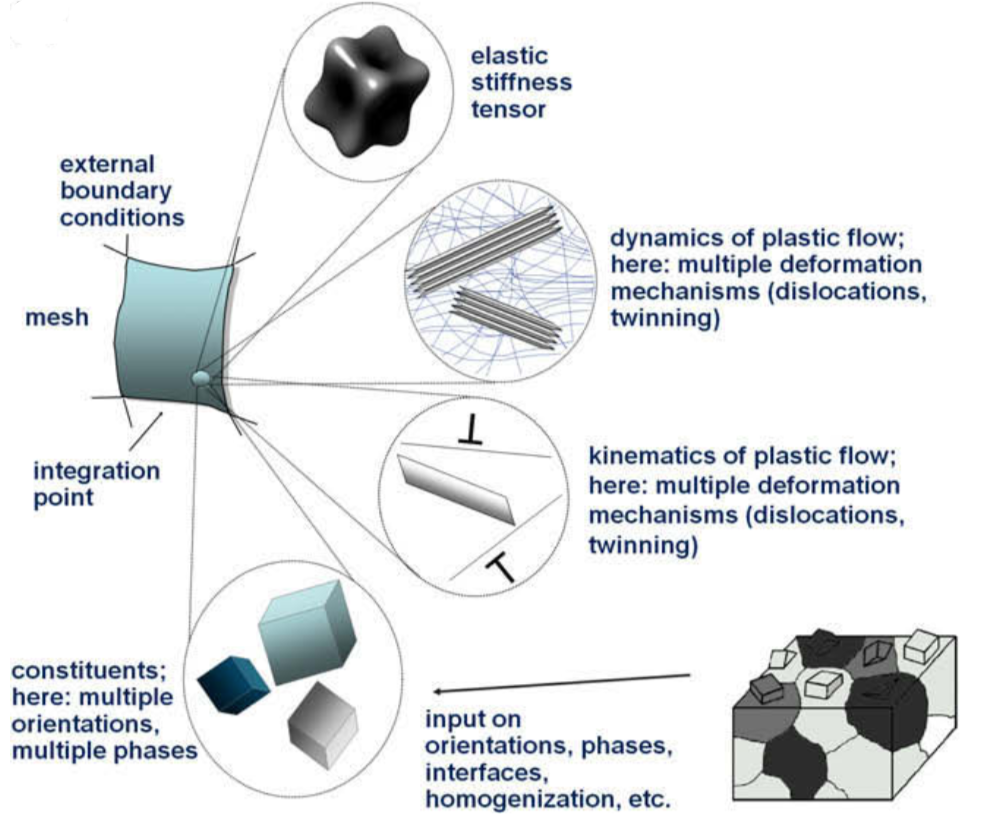
\includegraphics[width=1.0\textwidth]{cpfe.png}
	\hspace{1mm}
	\caption{Schematic representation of CPFE simulations \cite{ROTERS20101152}}  
	\label{fig:cpfe}
\end{figure}

The spatially resolved deformation simulations mentioned above provide high resolution information of the local deformation characteristics and have become the tool of choice for studying the effect of microstructure on the deformation behavior. These predictions are also compared with relevant experimental measurements, where available \cite{POKHAREL2019201} \cite{THOOL2020102785} \cite{Radhakrishnan_2000}. However, these methods generally have large associated computational costs, which may act as a deterrent for performing large number of simulations for advanced computational materials design and screening. In such scenarios, Machine Learning (ML) can be used to develop surrogate models and reduce the computational costs associated with these finite element models \cite{pandey2020machine} \cite{muhammad2020machine} \cite{shen2019convolutional} \cite{MANGAL2018122}.

Machine learning is an emerging research field and has been widely adopted in recent years due to it's outstanding ability to predict properties, relationships and inferences from different kinds of data, with relatively lower computational costs. In the past decade, a variety of surrogate models have been developed and implemented to predict the deformation characteristics of metallic systems. Mangal and Holm \cite{MANGAL2018122} used machine learning to predict the formation of stress hotspots in face centered cubic materials. They implemented a random forest algorithm, which is used for modeling classification and regression problems, in this case classifying grains as stress hotspots, where localized deformation may occur. The algorithm also successfully captured the effect of changing material and texture parameters on the stress hotspots. The model predicted stress hotspots with an accuracy of ~74\%, assuming FFT-based CP simulations as the ground truth. Muhammad et al. \cite{muhammad2020machine} implemented an Artificial Neural Network (ANN) model to predict the local strain distribution, fracture and evolution of plastic anisotropy in additvely manufactured alloys. They were able to predict the location, intensity and the shape of shear bands before failure with high accuracy. The implementation of Convolutional Neural Network (CNN) model has been successfully demonstrated by Beniwal et al. \cite{beniwal2019deep} for predictive modeling of structure-property linkages. This is a reduced order model which has the power to make predictions from just the microstructure image. Deep Learning (DL) based methods have been used to model reverse engineering problems such as using diffraction patterns to reconstruct microstructures \cite{shen2019convolutional}. Kotkunde et al. \cite{kotkunde2014prediction} demonstrated an ANN model to predict the forming limit diagram for sheet metals. A number of parameters such as tool and die geometry and working conditions dictate the sheet metal forming process. The ANN-based approach predicts the forming limit diagram at various combinations of process parameters, otherwise predicted with the help of FE simulations. 

\begin{figure}[!h]
	\centering
	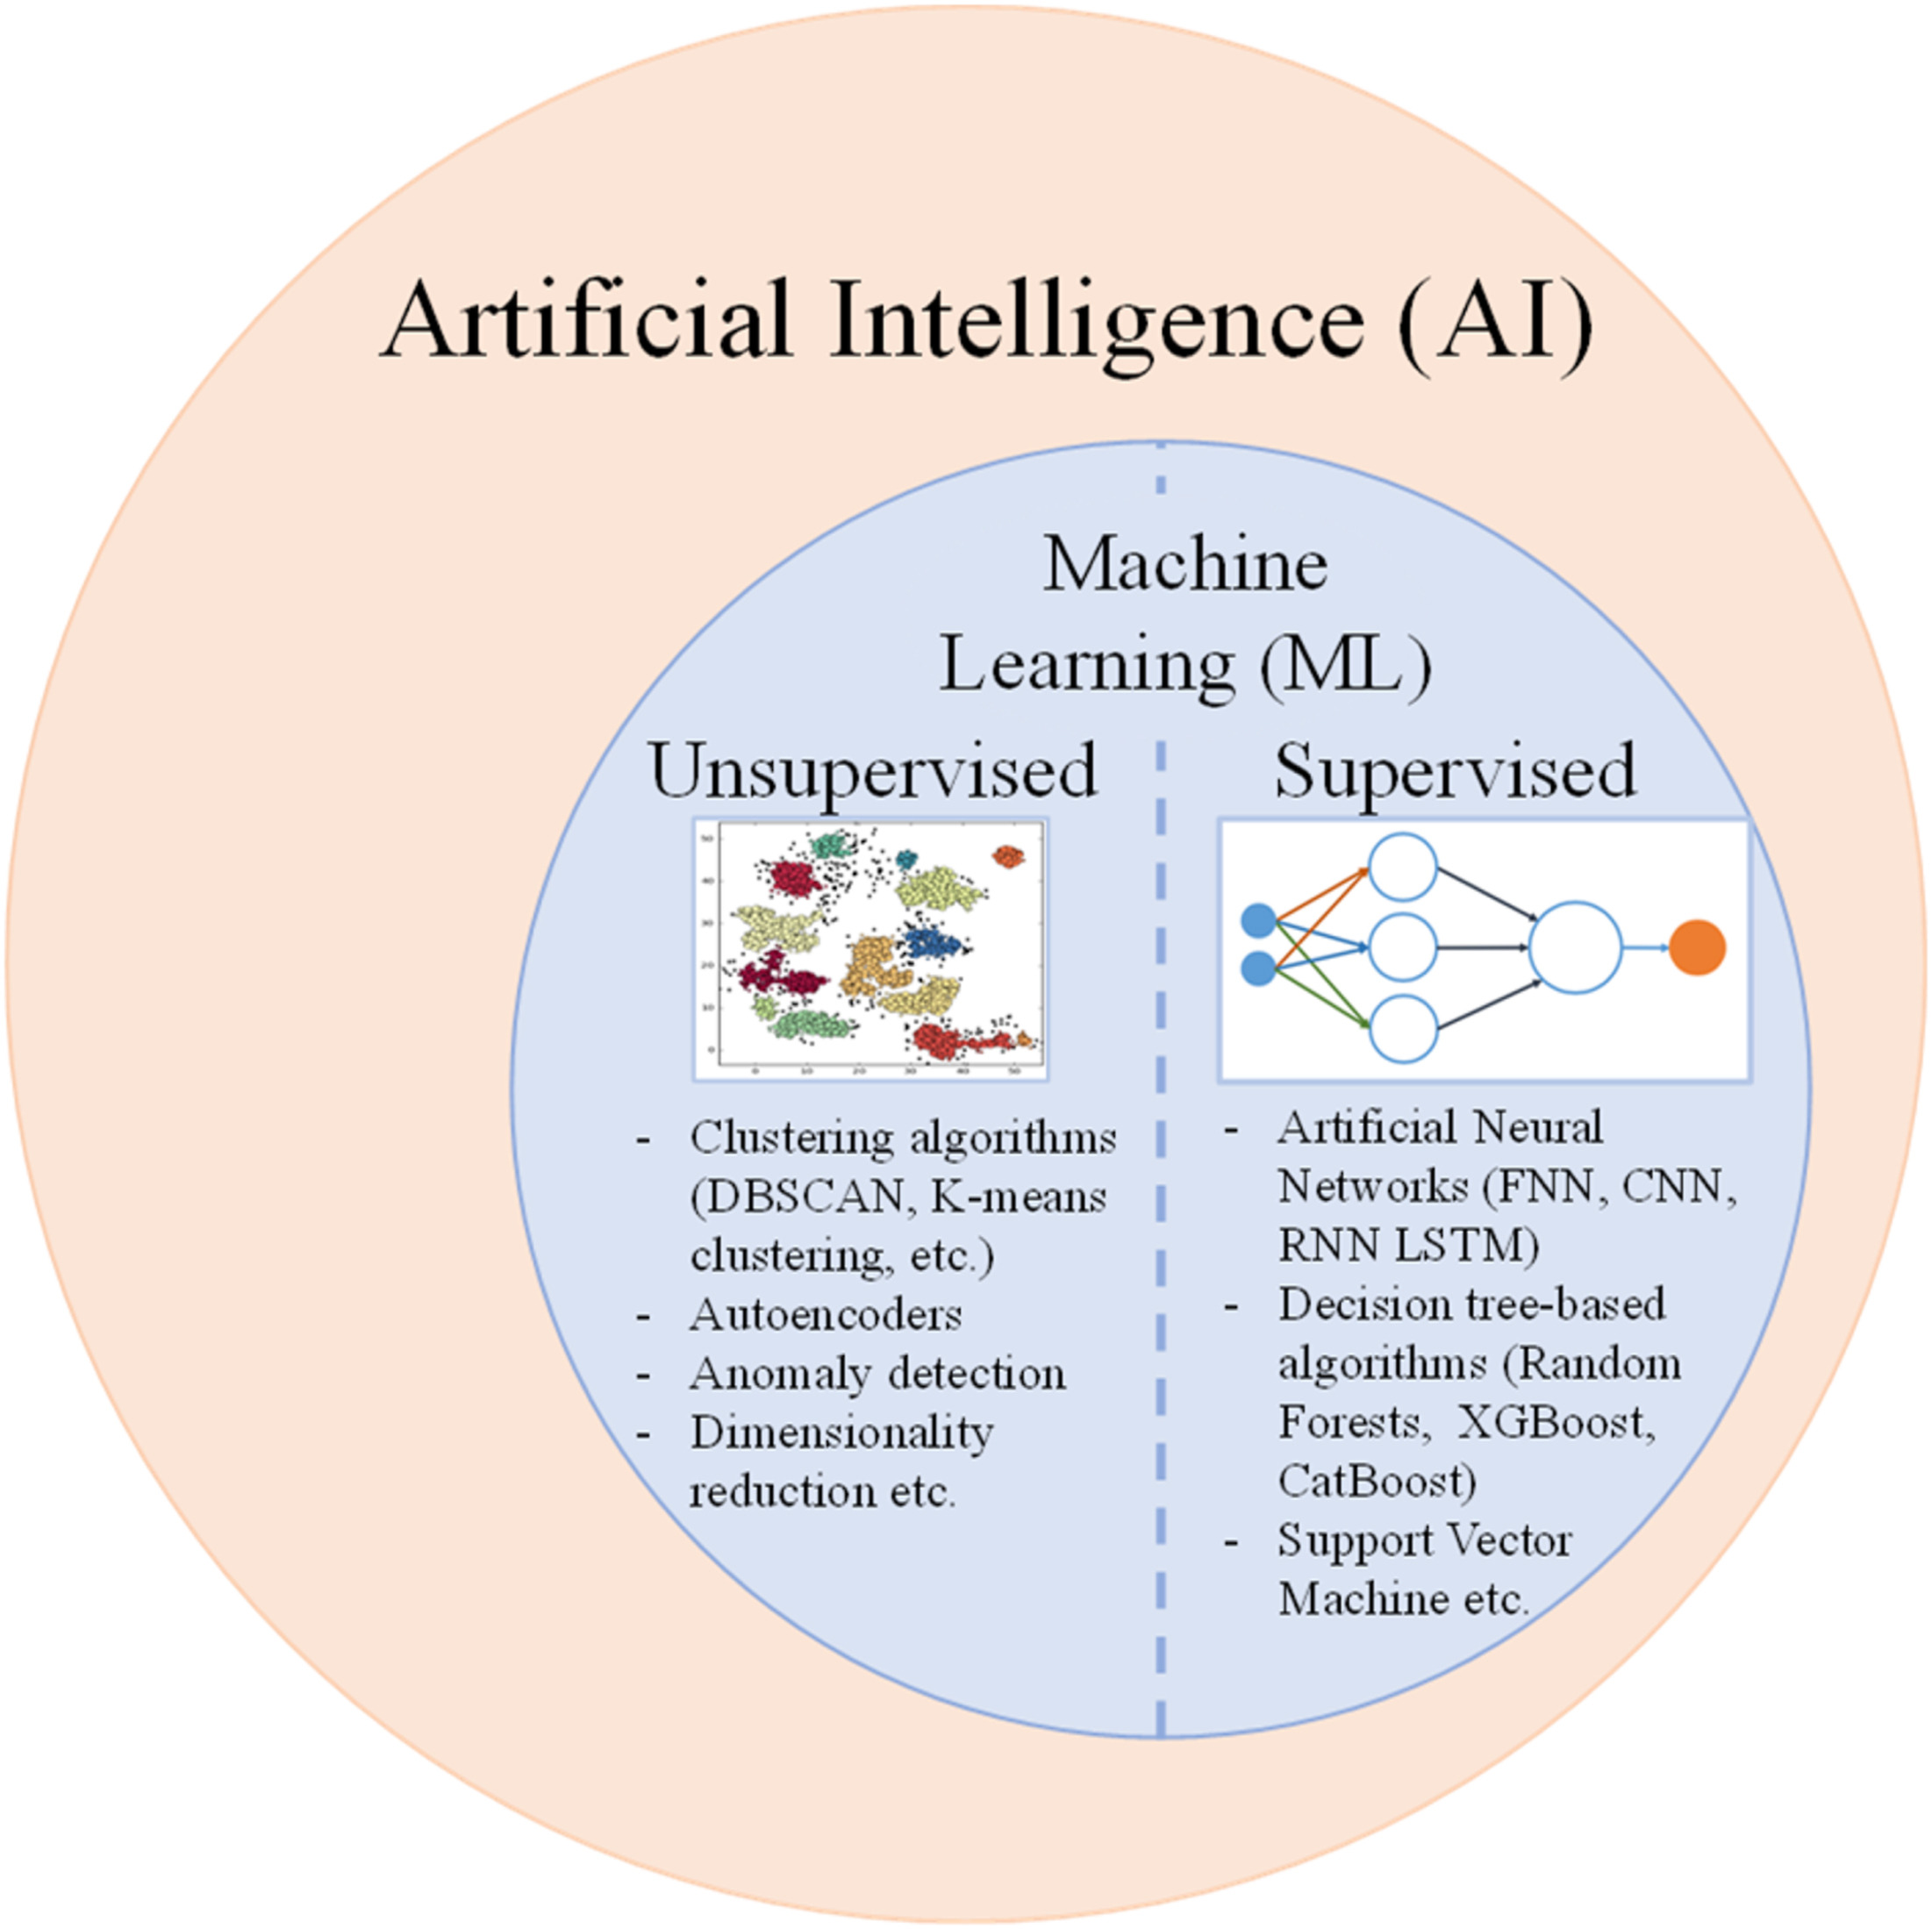
\includegraphics[width=0.7\textwidth]{ml-types.jpg}
	\hspace{1mm}
	\caption{Various types of machine learning models \cite{muhammad2020machine}.} 
	\label{fig:ml-types}
\end{figure}

Further, recurrent Neural Networks (RNN) have been widely for sequence modeling in various fields, but they have shown to be computationally expensive. Recently, a long-short term memory (LSTM) RNN network was proposed, which has the capability of remembering states over time and thus capable of modeling dynamic systems \cite{hochreiter1997long}. Pandey and Pokharel \cite{pandey2020machine} demonstrate a LSTM-based framework for predicting the microstructure evolution under tensile loading of polycrystalline materials. They used a first-order approximation by taking the effect of only nearest neighbor interactions on each crystalline point. Their model doesn't account for any long range interactions and yet produces results with 99\% accuracy. 

Figure \ref{fig:ml-types} shows the classification of some machine learning algorithms commonly used in materials science.

\section{Plan Of Thesis}
A systematic study of various deep learning techniques for predicting the evolution of the deformed microstructure a dual phase (DP) steel has been performed in this thesis. A dislocation density based J2 plasticity finite element framework is used to run deformation simulations of the two phase microstructures of dual phase steels. The J2 plasticity simulations are considered as the ground truth for developing the machine learning model. We start with an ANN and optimize the hyper parameters to achieve the best possible results. Further, as plastic deformation is a history-dependent process, LSTMs are better suited for modeling them as they have the capability to remember states over time. Hence, in the next approaches we show a vanilla LSTM and develop on it to improve our results. The data we are dealing with is spatio-temporal in nature. We demonstrate the ability of LSTM to deal with this kind of data and produce accurate results. 

The subject matter of the thesis is presented in the following 5 chapters:
\begin{itemize}
\item Chapter 2 discusses the fundamentals of deep learning, including the underlying theory of the algorithms used in our work. Further, we discuss some of the approaches used in the literature and their shortcomings.
\item Chapter 3 first provides a summary of the J2 plasticity model used for DP steels. We then discuss the ML model development and implementation.
\item Chapter 4 discusses preliminary results obtained from our model.
\item Chapter 5 summarizes the work done so far and provides details of work planned in the next phase.  
\end{itemize}